\section{Implementación}\label{sec:implementacion}

\begin{frame}{Diagrama UML}
    \begin{figure}[H]
        \centering
        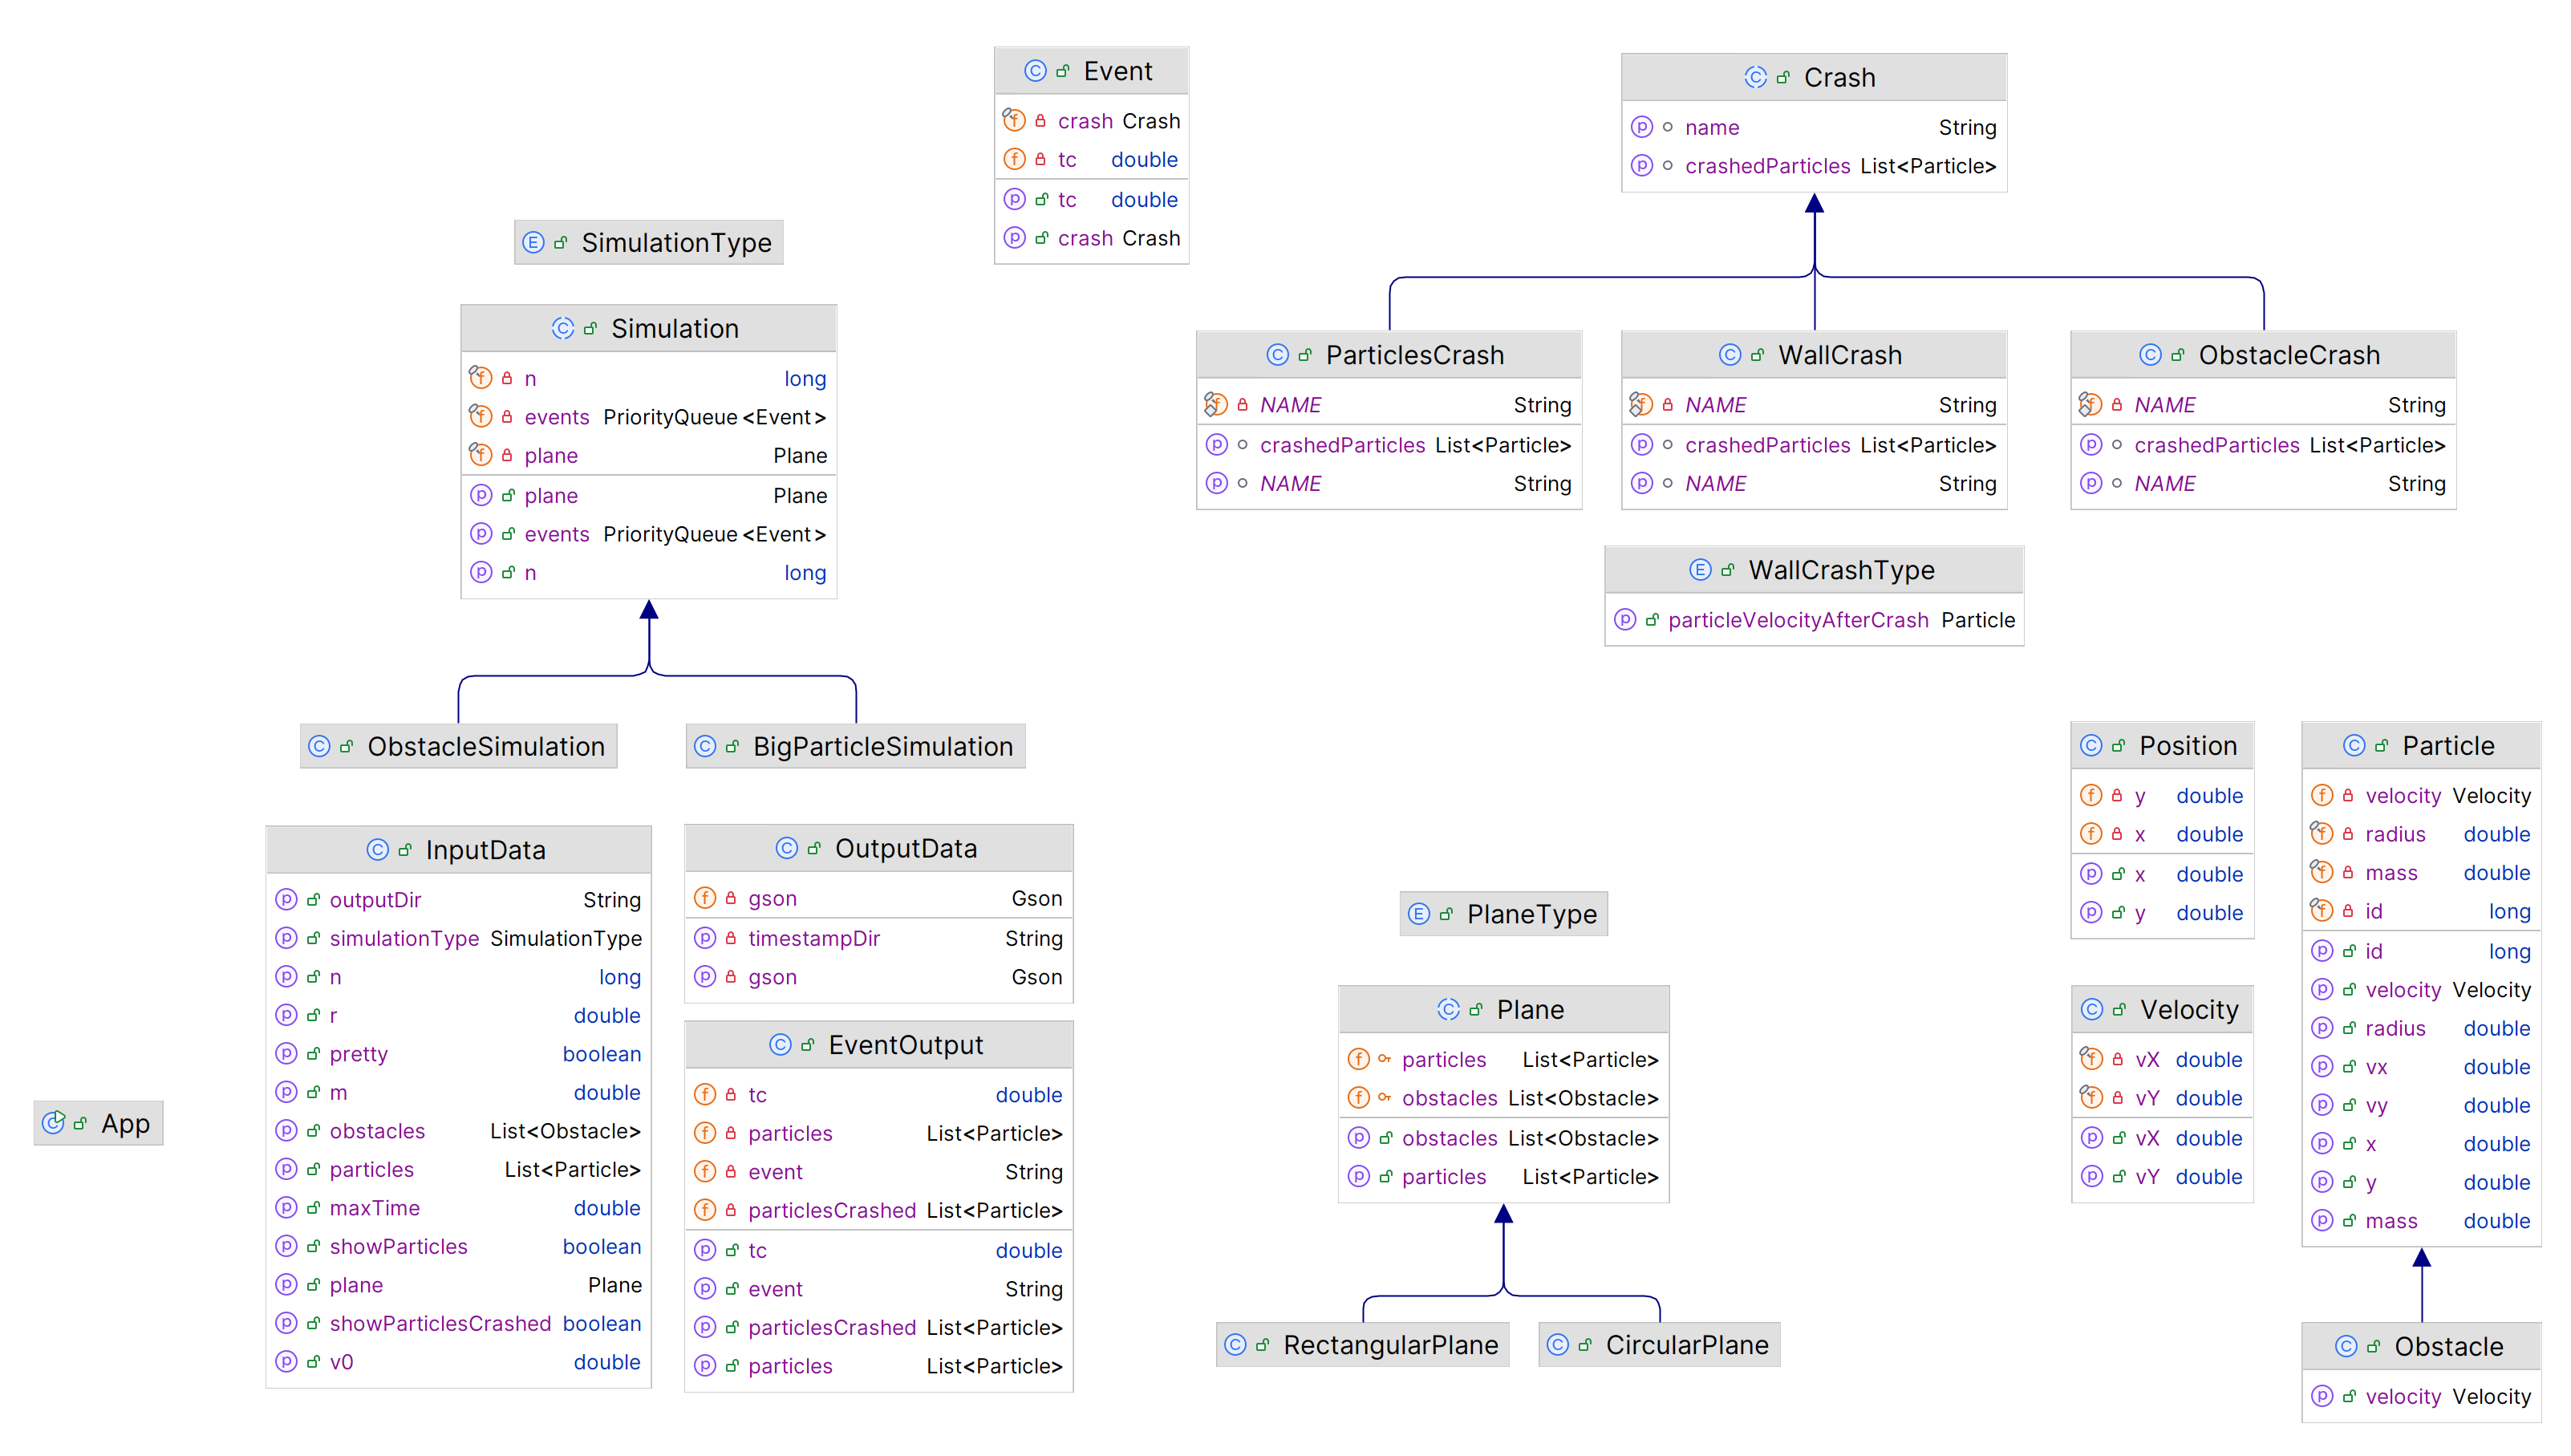
\includegraphics[width=0.8\linewidth]{pic/03-impl/UML}\label{fig:figure-uml}
    \end{figure}
\end{frame}

\begin{frame}{Pseudocódigo}
    \footnotesize{
    \begin{algorithmic}
        \State $queue = PriorityQueue()$
        \State \text{Crear n partículas con velocidad y dirección aleatoria}
        \For{\text{partícula i}}
            \State \text{Calcular tiempo de colisión con contorno, otras partículas y obstáculos}
            \State \text{Agregar eventos a $queue$}
        \EndFor
        \While{\text{$t$ < $t_{max}$}}
            \State \text{Obtener evento de $queue$}
            \State \text{Actualizar posiciones de las partículas}
            \State \text{Actualizar $t$}
            \State \text{Calcular la nueva velocidad de las partículas involucradas en la colisión}
            \State \text{Eliminar los eventos que involucran a las partículas colisionadas de $queue$}
            \For{\text{partícula colisionada}}
                \State \text{Calcular tiempo de colisión con contorno, otras partículas y obstáculos}
                \State \text{Agregar eventos a $queue$}
            \EndFor
        \EndWhile
    \end{algorithmic}
    }
\end{frame}


